\section{Prince of Persia}
Suponga que en un nivel del videojuego \emph{Prince of Persia (1989)} el protagonista
tiene que atravesar N baldosas consecutivas. Sobre cada baldosa pueden ocurrir una de
dos cosas:
\begin{enumerate}
	\item Hay un trampolín que le permite saltar una cantidad de baldosas entre
		2 y \texttt{jumpMax} hacia adelante. El príncipe puede decidir
		si usa el trampolín para saltar o si simplemente avanza a la
		siguiente baldosa.
	\item La baldosa es quebradiza y el príncipe se cae al abismo.
\end{enumerate}
Se debe desarrollar un programa que determine si existe alguna forma de llegar al
final del recorrido. Se debe llegar exactamente a la N-ésima baldosa porque
posteriormente sólo hay un abismo.
%
\subsection*{Ejemplo 1}
Suponiendo que cada posición se representa por la cantidad de baldosas que permite
saltar el trampolín que está en esa posición y -1 indica que en esa posición hay
una caída al abismo, el siguiente es un ejemplo en el que las casillas coloreadas
muestran cómo se podría llegar al final. Se colorean de amarillo las posiciones en
las que se debe caminar y en verde las posiciones en las que se debe saltar:

\medskip
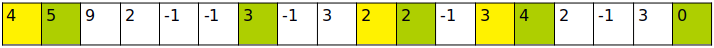
\includegraphics[width=0.75\textwidth]{propYes.png}
%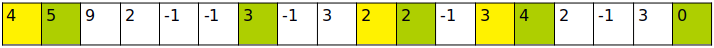
\includegraphics[]{propYes.png}
%
\subsection*{Ejemplo 2}
Por el contrario, para el siguiente ejemplo no es posible llegar al final:

\medskip
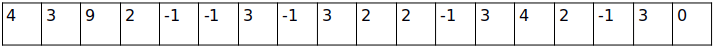
\includegraphics[width=0.75\textwidth]{propNo.png}
%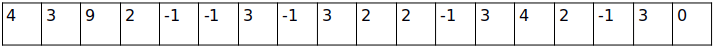
\includegraphics[]{propNo.png}
